% !TEX encoding = UTF-8
% !TEX TS-program = pdflatex
% !TEX root = ../tesi.tex

%**************************************************************
\chapter{Progettazione e codifica}
\label{cap:progettazione-codifica}
%**************************************************************

\intro{Il capitolo approfondisce l'architettura del software prima complessivamente e poi nel dettaglio, descrivendo i problemi incontrati e la soluzione applicata.}\\

\section{Architettura generale}

Il modulo è stato progettato tenendo a mente i requisiti di scalabilità imposti dall'azienda. L'architettura è stata principalmente definita durante le prime settimane ma ha subito modifiche anche in corso d'opera in risposta ai bisogni ed alle difficoltà rilevati.


\begin{figure}[!h] 
    \centering 
    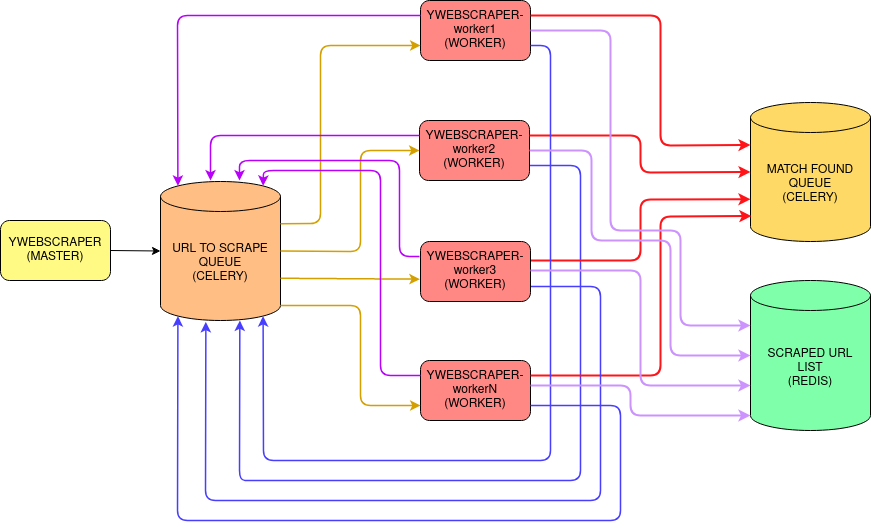
\includegraphics[width=1\columnwidth]{chapter4-project/architettura-generale.png} 
    \caption{Architettura generale.}
\end{figure}